Após a construção da ISS, surgiu a necessidade de \textit{berthing} (atracação) para módulos de carga como o HTV (Japão) e Cygnus (EUA), que utilizavam sistemas robóticos, como o Canadarm2 para atracar módulos e veículos.

\subsection{Cygnus}
A atracação (berthing) da espaçonave Orbital Cygnus à Estação Espacial Internacional (ISS) representa um marco significativo na colaboração entre agências espaciais e empresas privadas para o avanço das operações em órbita baixa. A Orbital Cygnus é um veículo de reabastecimento não tripulado desenvolvido pela Northrop Grumman para transportar cargas essenciais, como suprimentos, equipamentos e experimentos científicos, para a ISS. Durante essas missões, a Cygnus se aproxima da estação e é capturada pelo braço robótico Canadarm2, operado pelos astronautas a bordo da ISS, que finalizam o processo de atracação conectando a espaçonave a um dos módulos da estação \cite{nasaCygnus}.

\begin{figure}[H]
    \centering
    \includegraphics[width=0.75\linewidth]{RevDaLiteratura/Imagens/Cygnus Northrop Grumman.png}
    \caption{Espaçonave cargueira Cygnus e o Canadaarm2. Fonte: NASA.}
    \label{fig:CygnusFoto}
\end{figure}

A capacidade da Cygnus de realizar missões regulares de reabastecimento destaca a importância de parcerias público-privadas no suporte contínuo às operações da ISS. Essas missões não apenas garantem o fornecimento de recursos críticos, mas também reforçam a infraestrutura para conduzir pesquisas científicas de ponta em microgravidade. A flexibilidade e eficiência do design da Cygnus permitem que ela transporte uma ampla variedade de cargas, desde experimentos científicos avançados até equipamentos necessários para a manutenção da ISS \cite{nasaCygnusDeparture}. Além disso, o sucesso dessas missões demonstra a maturidade e a confiabilidade dos sistemas de berthing, que são cruciais para futuras operações espaciais, incluindo estações espaciais comerciais e missões no espaço profundo \cite{nasaCygnus}.

O papel do Canadarm2 no processo de berthing reflete o alto nível de integração tecnológica necessário para operações complexas em órbita. O braço robótico não apenas captura a Cygnus, mas também facilita o acoplamento seguro, permitindo que a tripulação acesse os suprimentos transportados. Esse processo combina automação avançada com intervenção humana precisa, destacando a sinergia entre os sistemas robóticos e os operadores humanos em operações espaciais \cite{nasaCygnus}.

A atracação da Cygnus à ISS simboliza o progresso contínuo na exploração espacial e o sucesso de modelos colaborativos que integram inovação tecnológica, capacidade operacional e parceria internacional. À medida que novas missões são planejadas, a experiência adquirida com o berthing da Cygnus será fundamental para enfrentar os desafios das próximas gerações de operações espaciais \cite{nasaCygnus}.

\subsection{HTV}
Em setembro de 2009, o Japão alcançou um marco histórico em seu programa espacial ao lançar o HTV-1 (H-II Transfer Vehicle), sua primeira missão de reabastecimento para a Estação Espacial Internacional (ISS). Desenvolvido pela Agência de Exploração Aeroespacial do Japão (JAXA), o HTV-1 foi projetado para transportar cargas essenciais, incluindo alimentos, equipamentos e experimentos científicos, para os módulos da estação. O lançamento, realizado por meio de um foguete H-IIB a partir do Centro Espacial de Tanegashima, destacou a crescente capacidade tecnológica do Japão em operações espaciais complexas e sua contribuição significativa ao programa da ISS \cite{nasaHTV}.

\begin{figure}[H]
    \centering
    \includegraphics[width=0.75\linewidth]{RevDaLiteratura/Imagens/HTV Japan.png}
    \caption{O HTV e o Canadaarm2. Fonte: NASA.}
    \label{fig:HTVfoto}
\end{figure}

O HTV-1 utilizou uma abordagem inovadora para se aproximar da ISS. Diferentemente de sistemas automáticos de docking, a espaçonave foi projetada para realizar um processo de berthing, no qual ela se aproximava cuidadosamente da estação, sendo capturada pelo braço robótico Canadarm2, operado pelos astronautas a bordo. Após a captura, o HTV-1 foi conectado a um dos módulos da ISS para permitir o acesso à carga. Essa missão inaugural demonstrou a eficiência do sistema de berthing e a confiabilidade do veículo, abrindo caminho para uma série de missões subsequentes \cite{nasaHTV}.

Além de sua capacidade de transporte, o HTV-1 foi um exemplo de cooperação internacional na exploração espacial. A missão reforçou a parceria do Japão com outras agências espaciais, incluindo a NASA, e destacou o papel essencial da JAXA no suporte à ISS. A contribuição japonesa foi ainda mais significativa devido à capacidade do HTV de transportar cargas maiores do que outras espaçonaves de reabastecimento na época (5.896 kg), como a Cygnus (5.000 kg) \cite{northropCygnusFactsheet} ou a Progress (2.100 kg) \cite{russianspacewebProgress}. Essa flexibilidade permitiu à ISS receber equipamentos volumosos e experimentos que eram críticos para a continuidade de operações científicas em microgravidade \cite{nasaHTV}.

\subsection{Canadarm2}

O Canadarm2, um braço robótico avançado a bordo da Estação Espacial Internacional (ISS), desempenha um papel essencial nas operações da estação. Ele foi desenvolvido pela Agência Espacial Canadense (CSA), e foi lançado em 2001 como parte da contribuição do Canadá para a ISS. Este equipamento sofisticado é utilizado para uma variedade de tarefas críticas, incluindo o acoplamento e desacoplamento de espaçonaves de reabastecimento, manutenção de componentes externos da estação e suporte a atividades extraveiculares realizadas pelos astronautas. Sua capacidade de se mover ao longo da estrutura da ISS, conectando-se a diferentes pontos de ancoragem, proporciona uma flexibilidade única nas operações em órbita \cite{canadarm2}.

\begin{figure}[H]
    \centering
    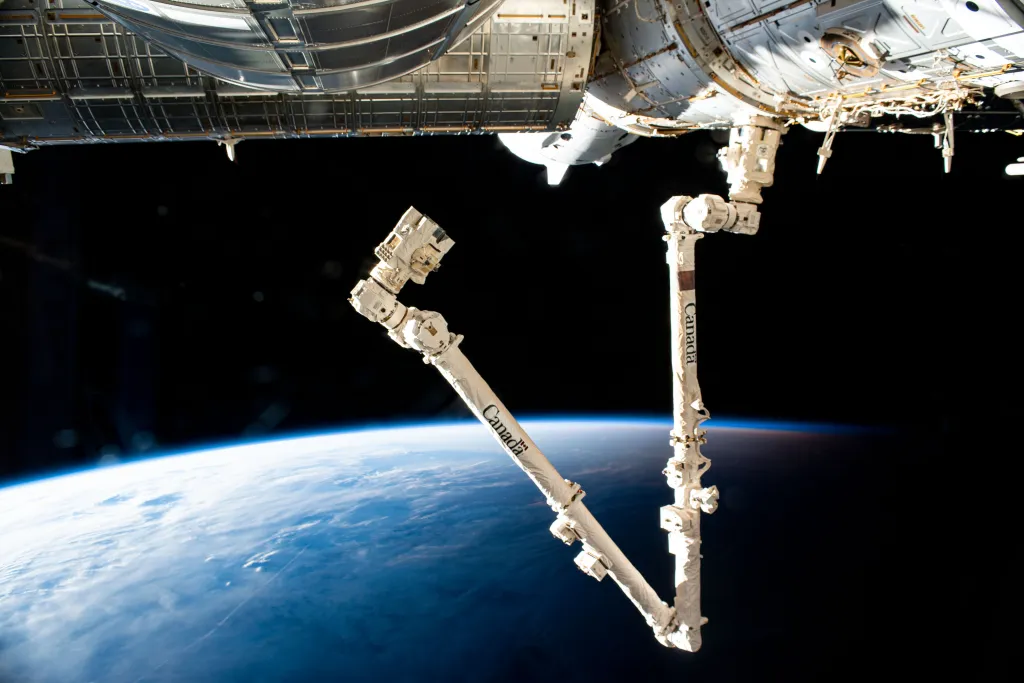
\includegraphics[width=0.75\linewidth]{RevDaLiteratura/Imagens/Canadarm2.png}
    \caption{Canadarm2. Fonte: NASA.}
    \label{fig:Canadaarm2Foto}
\end{figure}


O Canadarm2 mede 17,6 metros de comprimento e possui sete articulações que permitem uma ampla gama de movimentos. Ele é controlado tanto pelos astronautas a bordo da ISS quanto pelos operadores em terra, demonstrando a integração entre automação e supervisão humana. Além disso, sua tecnologia avançada permite a manipulação precisa de cargas pesadas e delicadas, essencial para operações como a captura de espaçonaves de reabastecimento, como a Cygnus e o HTV \cite{canadarm2}.

\subsection{Progress}

A Progress é uma espaçonave não tripulada desenvolvida pela Rússia para missões de reabastecimento à Estação Espacial Internacional (ISS) e anteriormente às estações espaciais soviéticas, como a Salyut e a Mir. Desde seu primeiro voo em 1978, a Progress tem desempenhado um papel crucial na logística de missões em órbita baixa, transportando suprimentos essenciais, incluindo alimentos, água, oxigênio, equipamentos e combustível para as estações espaciais. Além de seu papel como veículo de reabastecimento, a Progress também é usada para remover resíduos da ISS, contribuindo significativamente para a manutenção operacional da estação \cite{progress}.

\begin{figure}[H]
    \centering
    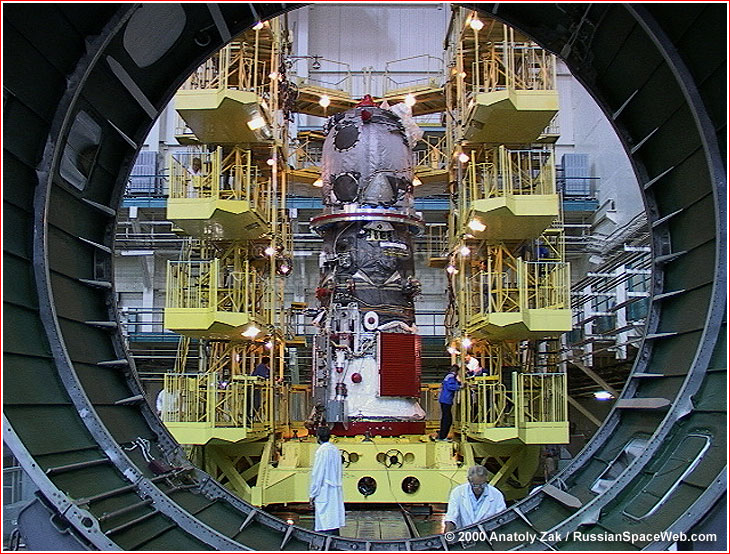
\includegraphics[width=0.75\linewidth]{RevDaLiteratura/Imagens/Progress.jpg}
    \caption{Espaçonave Progress em construção. Fonte: RussianSpaceWeb.}
    \label{ProgressFoto}
\end{figure}

A espaçonave Progress é baseada no design da nave Soyuz, com algumas modificações para atender às suas funções específicas. Ela consiste em três módulos principais: um módulo de carga pressurizado, um tanque de combustível não pressurizado e um módulo de propulsão. Esse design permite que a Progress transporte tanto carga seca quanto líquidos, otimizando sua utilidade em missões de reabastecimento. Após completar sua missão, a Progress é deliberadamente desacoplada e destruída durante a reentrada na atmosfera terrestre, queimando junto com os resíduos coletados da estação \cite{progress}.

A confiabilidade e eficiência da Progress a tornaram um dos pilares do suporte à ISS, permitindo entregas regulares de suprimentos e garantindo a continuidade das operações científicas e habitacionais em órbita. Suas missões são lançadas a partir do cosmódromo de Baikonur utilizando foguetes Soyuz, demonstrando a integração de longa data entre diferentes elementos do programa espacial russo. A Progress também tem servido como um veículo de teste para novas tecnologias, incluindo sistemas de automação e melhorias nos sistemas de acoplamento, reforçando sua importância estratégica no programa espacial \cite{progress}.

Ao longo das décadas, a Progress consolidou seu papel como uma espaçonave essencial para o sucesso das operações da ISS. Sua capacidade de transportar grandes volumes de carga, aliada à sua simplicidade operacional, a torna uma solução eficiente para o suporte logístico de longo prazo em órbita terrestre. O legado da Progress continua a influenciar o design e a operação de veículos espaciais de reabastecimento modernos, destacando sua contribuição duradoura para a exploração espacial \cite{progress}.

\subsection{ATV}

O Automated Transfer Vehicle (ATV) foi um veículo de reabastecimento não tripulado desenvolvido pela Agência Espacial Europeia (ESA) para apoiar as operações da Estação Espacial Internacional (ISS). Lançado pela primeira vez em 2008, o ATV foi projetado para transportar suprimentos essenciais, como alimentos, água, oxigênio e equipamentos científicos, além de combustível para reabastecer os sistemas de propulsão da ISS. Com um design inovador e altamente automatizado, o ATV também desempenhava um papel crucial ao utilizar seus próprios motores para ajustar a órbita da ISS, garantindo sua estabilidade e mitigando o impacto da resistência atmosférica \cite{esaATV}.

Cada missão do ATV era composta por uma espaçonave descartável lançada a partir do foguete Ariane 5, que transportava até sete toneladas de carga útil. O ATV era equipado com sistemas automáticos de navegação e acoplamento que permitiam conectar-se à ISS sem a necessidade de intervenção humana direta. Essa capacidade de automação destacava o avanço tecnológico europeu em operações espaciais complexas. Após completar sua missão, o ATV era desacoplado da estação e direcionado para reentrada controlada na atmosfera terrestre, onde era destruído junto com resíduos descartados da ISS \cite{esaATV}.

O programa ATV foi um marco significativo na colaboração internacional em exploração espacial. Ao longo de suas cinco missões bem-sucedidas entre 2008 e 2015, o ATV demonstrou a capacidade da Europa de contribuir com tecnologias avançadas para a ISS, fortalecendo parcerias com outras agências espaciais, como a NASA e a Roscosmos. Além de suas funções operacionais, o ATV serviu como plataforma de teste para novas tecnologias que poderiam ser aplicadas em futuras missões espaciais, incluindo exploração em espaço profundo \cite{esaATV}.

\subsection{Avanços tecnológicos}

O ATV em sua última missão, realizada pelo ATV-5 Georges Lemaître em 2015, consolidou o sucesso de seu sistema automatizado de atracação, sem necessidade de intervenção humana direta. Equipado com sistemas de navegação precisos, o ATV utilizava sensores de laser e câmeras para determinar sua posição e orientação em relação à Estação Espacial Internacional (ISS), permitindo que o veículo realizasse manobras autônomas complexas até se conectar com segurança à estação \cite{esaATVFinal}.

A automação do ATV não apenas garantiu a precisão do processo de acoplamento, mas também reduziu significativamente os riscos associados a erros humanos. Durante suas missões, o ATV demonstrou ser capaz de operar de forma independente em todas as fases críticas, desde a aproximação inicial até o contato final com a ISS. Essa tecnologia avançada permitiu uma integração perfeita entre o veículo e a estação, sem a necessidade de assistência constante da tripulação ou de controladores em terra. A confiabilidade desse sistema automatizado foi um marco importante para a exploração espacial, estabelecendo novos padrões para veículos de reabastecimento em missões futuras \cite{esaATVFinal}.

A última missão do ATV-5 reafirmou a viabilidade e o sucesso de sistemas de automação completa em operações espaciais. A experiência adquirida com o ATV servirá como base para o desenvolvimento de novas gerações de veículos espaciais automatizados, reforçando a importância de tecnologias independentes para missões em ambientes desafiadores, como o espaço profundo. O legado do ATV como pioneiro na automação continua a influenciar o design de veículos espaciais modernos \cite{esaATVFinal}.

\subsection{Rendezvous and docking automáticos}

O Automated Transfer Vehicle (ATV) demonstrou uma capacidade avançada de rendezvous no espaço, destacando-se como um dos sistemas automatizados mais sofisticados desenvolvidos pela Agência Espacial Europeia (ESA). A aproximação do ATV à Estação Espacial Internacional (ISS) foi completamente autônoma, utilizando uma combinação de sensores avançados, software robusto e sistemas de controle de alta precisão. Durante cada missão, o ATV seguiu uma série de manobras planejadas, ajustando sua posição e velocidade com base em dados em tempo real, garantindo um rendezvous seguro e eficiente \cite{esaATVRendezvous}.

\begin{figure}
    \centering
    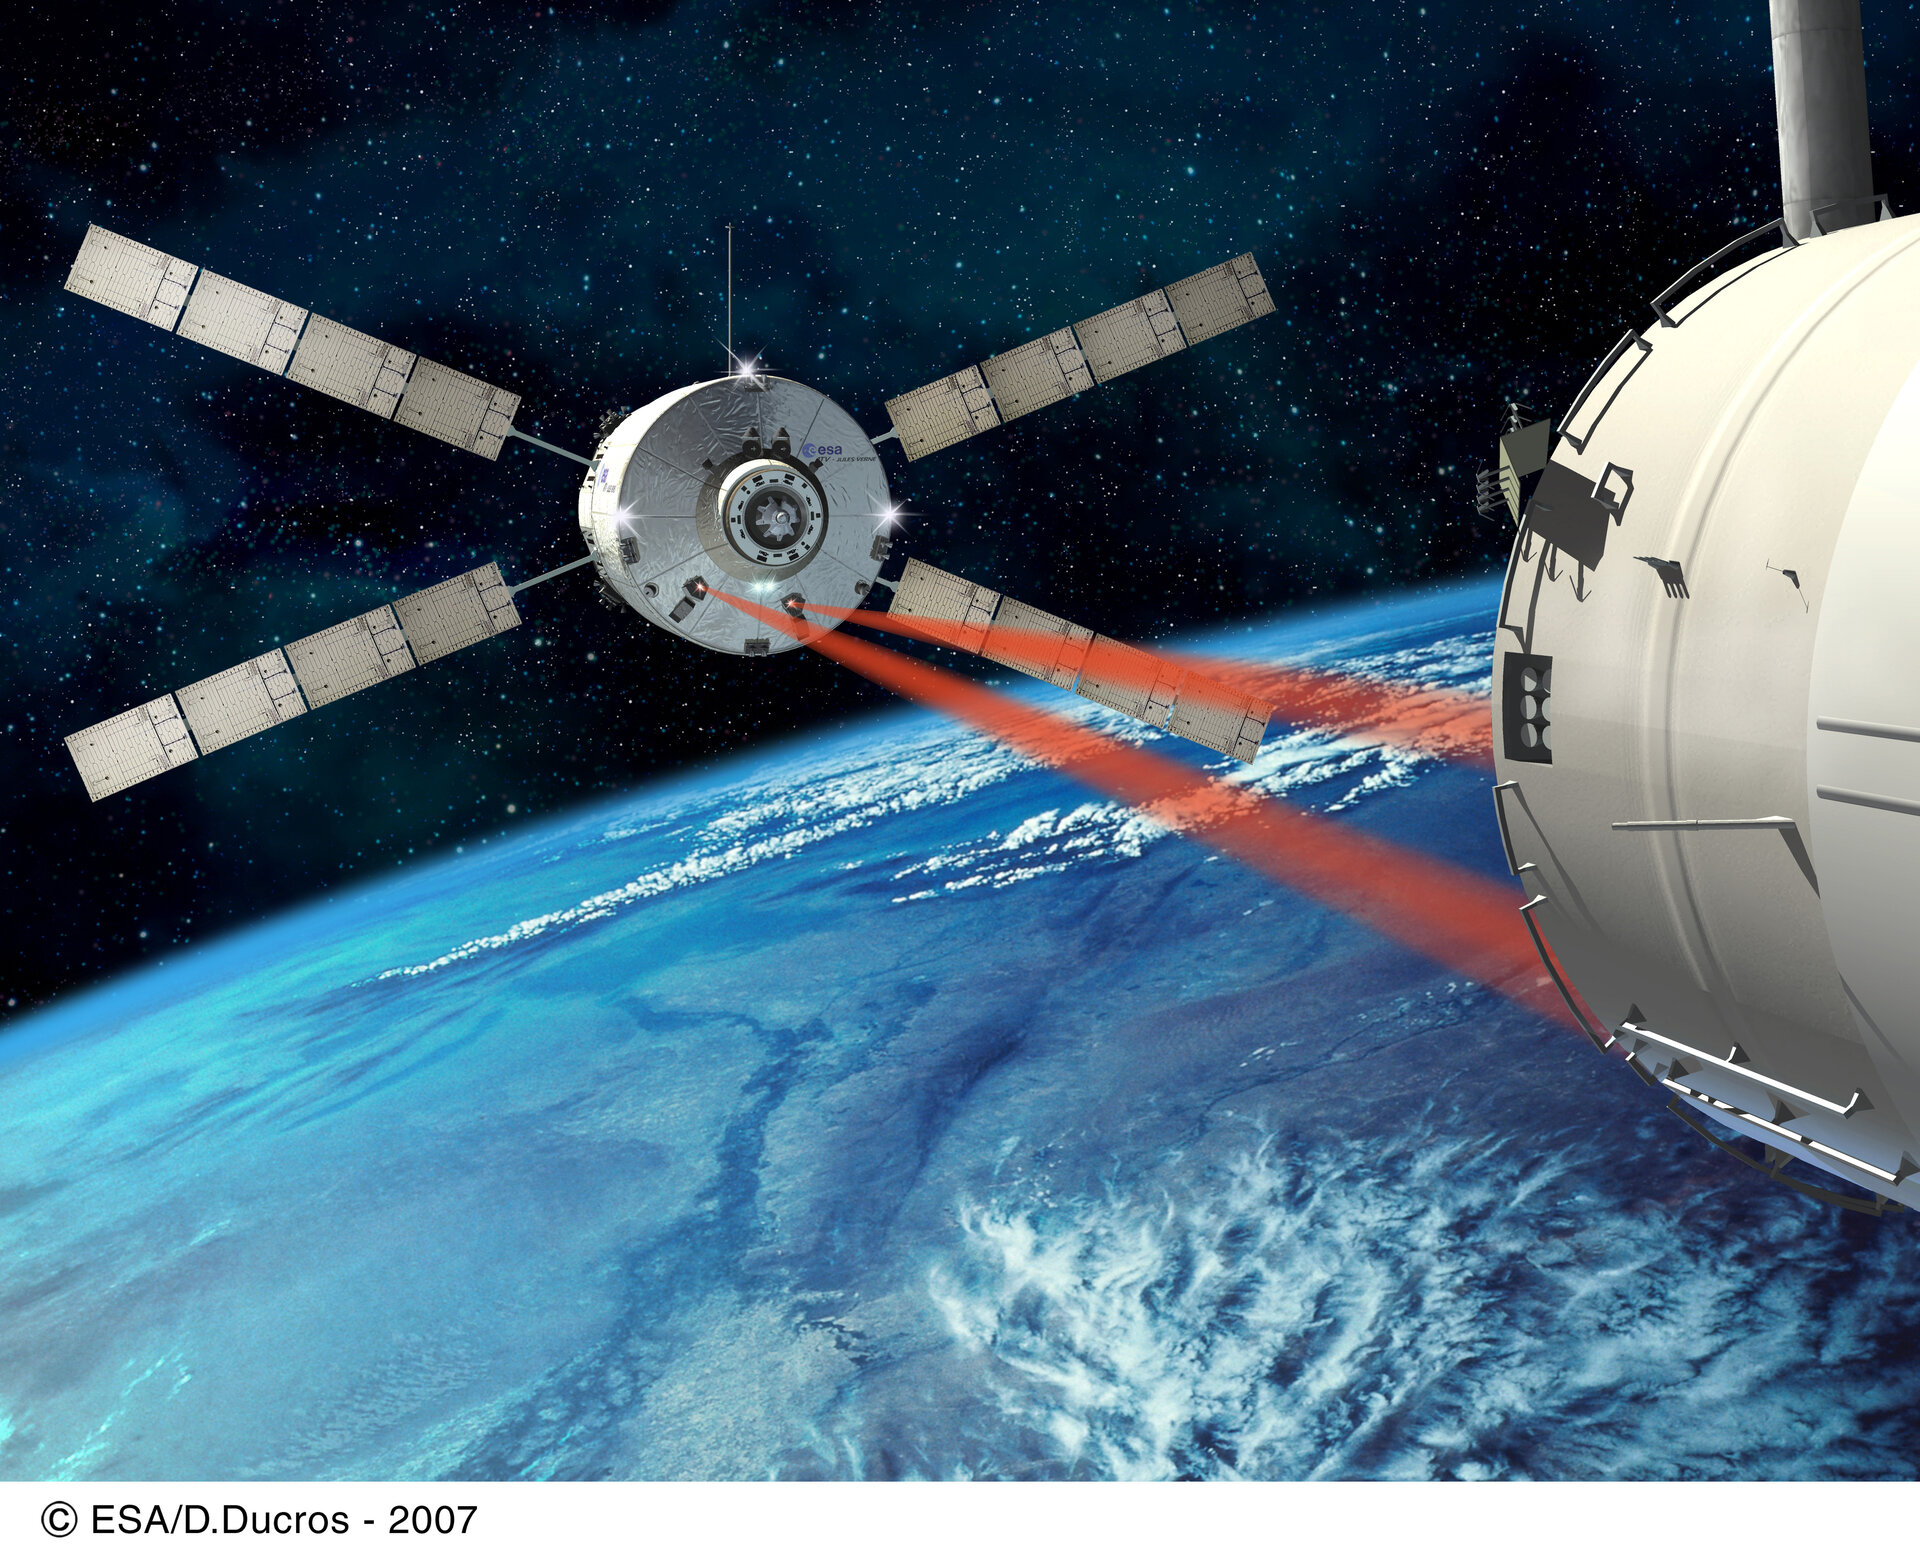
\includegraphics[width=0.75\linewidth]{RevDaLiteratura/Imagens/ATV RVD.jpg}
    \caption{Simulação da espaçonave ATV realizando rendezvous. Fonte: ESA.}
    \label{fig:ATVAutoDocking}
\end{figure}


O sistema de navegação do ATV era composto por sensores de laser, GPS e câmeras, que trabalhavam em conjunto para fornecer informações detalhadas sobre a posição relativa e a orientação da espaçonave em relação à ISS. Esses dados permitiam ajustes contínuos na trajetória do ATV, alinhando-o precisamente com a porta de acoplamento da estação. A automação completa do processo minimizava a necessidade de intervenção humana, tornando-o confiável e reduzindo o risco de erro \cite{esaATVRendezvous}.

Durante a fase final do rendezvous, o ATV utilizava um sistema de guia a laser para medir com precisão a distância e a orientação em relação à ISS. Essa tecnologia era essencial para as etapas finais, onde pequenos ajustes eram realizados para alinhar o ATV com o porto de acoplamento. A ESA desenvolveu algoritmos sofisticados para garantir que o processo fosse concluído com segurança, mesmo em cenários de falha parcial de sensores ou sistemas \cite{esaATVRendezvous}.

As missões do ATV demonstraram que sistemas de rendezvous totalmente automatizados são viáveis e eficazes para operações orbitais. Essa experiência abriu caminho para o desenvolvimento de tecnologias de navegação e acoplamento que podem ser aplicadas em futuras missões espaciais, incluindo aquelas destinadas à exploração de espaço profundo. O sucesso do ATV ressalta o papel fundamental da automação na expansão das capacidades humanas no espaço \cite{esaATVRendezvous}.















